\documentclass{article}
\usepackage{tikz}
\usepackage{amsmath}
\usetikzlibrary{matrix,arrows}

\begin{document}

\[
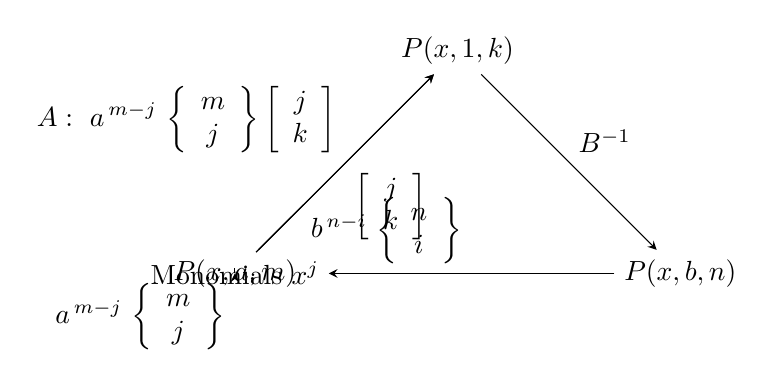
\begin{tikzpicture}[>=stealth, node distance=4cm, auto]
  % Nodes
  \node (Pa) {$P(x,a,m)$};
  \node (P1) [above right of=Pa] {$P(x,1,k)$};
  \node (Pb) [below right of=P1] {$P(x,b,n)$};
  \node (Mono) [below left of=P1] {Monomials $x^j$};

  % Arrows
  \draw[->] (Pa) -- node[above left] {$A:\ a^{\,m-j}\,\left\{\begin{array}{c} m \\ j \end{array}\right\} \left[\begin{array}{c} j \\ k \end{array}\right]$} (P1);
  \draw[->] (P1) -- node[above right] {$B^{-1}$} (Pb);
  \draw[->] (Pa) -- node[below left] {$a^{\,m-j}\,\left\{\begin{array}{c} m \\ j \end{array}\right\}$} (Mono);
  \draw[->] (Mono) -- node[below right] {$\left[\begin{array}{c} j \\ k \end{array}\right]$} (P1);
  \draw[->] (Pb) -- node[above left] {$b^{\,n-i}\,\left\{\begin{array}{c} n \\ i \end{array}\right\}$} (Mono);
\end{tikzpicture}
\]

\[
S_{m,n}(a,b) = \sum_{k=n}^m (a-b)^{\,m-k}
\left\{\begin{array}{c}m\\k\end{array}\right\}
\left[\begin{array}{c}k\\n\end{array}\right]
\]

\end{document}